\begin{appendices}
\chapter{- Introduction to Machine Learning}\label{appx:introMachineLearning}

\section{Heaviside Function}\label{appx:sec:heaviside}

The Heaviside step function is defined as
\begin{equation}\label{eq:heavisideDefintion}
h(z) =
\begin{cases}
&0 \ \mbox{if} \ z<0 \\
&\frac{1}{2} \ \mbox{if} \ z=0 \\
&1 \ \mbox{if} \ z>0.
\end{cases}
\end{equation}

and the relation between the logistic function and the heaviside function is
\begin{equation}
 \ H(z) = \lim_{k \to \infty} \left(\frac{1}{2} + \frac{1}{2}\tanh(kz) \right) = \lim_{k \to \infty} \left(\frac{1}{1+e^{-kz}} \right)
\end{equation}

Note in this sense that for a binary classification problem, the heaviside function \cref{eq:heavisideDefintion} is more appealing to the task, although its singularity at $z=0$ is problematic for optimization routines.

\section{Details of the log loss functions}\label{appx:sec:loglossDetails}

In \cref{figure-logLossValues} we display the values of the log loss function for different input probabilities:

\begin{figure}[h!]
\begin{center}
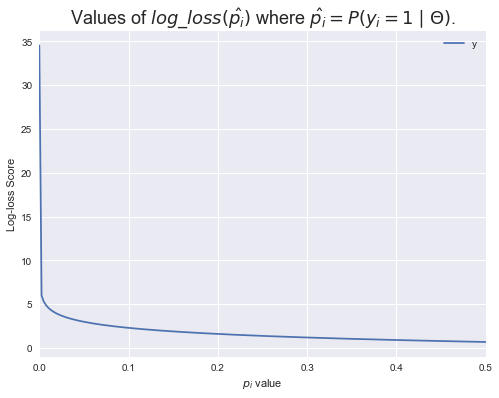
\includegraphics[width=0.7\columnwidth]{figures/logloss/figure-logLossValues.png}
\caption{ Error score series plot for the log loss function.
Different $p_i$ input values are displayed with their output log loss score.}
\label{figure-logLossValues}
\end{center}
\end{figure}

We have that it is a negative, concave, monotone increasing function with the estimated probability output by the classifier.
Also, the function is heavier for small probability values near zero than it is positive for large values near one.
This means that it penalizes strongly on wrong predictions; samples where the algorithm has a strong confidence in the prediction yet has misclassified.
This properties can be taken into advantage during the optimization procedure, which will always converge to a global optima.

Also, explicit forms can be given for the gradient and the Hessian of the loss function with regard to the whole dataset $X$ as a sum involving individual samples $x$.

The negative gradient can be analytically expressed in the following way: %can thus be analytically expressed
\begin{equation}
- \nabla l(\theta) = \sum_{i=1}^N (y_i - P(y_i \mid x_i,\theta))\cdot x_i = \textbf{X}^{\intercal}(\textbf{y}-\textbf{p})
\label{eq:logitHessian1}
\end{equation}
whilst the Hessian takes the following form:
\begin{equation}
\frac{\partial^2 l(\theta)}{\partial \theta \partial \theta^\intercal} = \sum_{i=1}^N x_i \cdot x_i^\intercal P(y_i \mid x_i,\theta)(1 -P(y_i \mid x_i,\theta))
\label{eq:logitHessian2}
\end{equation}

With this formulation, we can take any optimization procedure that benefits from the closed-form representations of the first and second derivatives of the loss function.



\chapter{Model Selection}

\section{Bias and variance errors in other loss functions}\label{appx:sec:biasVarianceExtensionLoss}

The work in~\cite{james-biasVarianceGeneral} defines what properties should be displayed by the bias and variance of an estimator in the general case.

For this, they define the systematic value of a random variable with respect to a loss function.


\begin{definition}{Systematic Value:}
Given a training set $\mathcal{T}$, a loss function $L(\cdot)$ and a random variable $Z$, the systematic value or systematic component of this variable is
$$ SZ =  \argmin_u \Expect_{Z} \left[ L(u,Z) \right]$$
\end{definition}

The systematic value is the nearest constant value to the random variable, with the measure as given by the loss function.
In this definition we are implicitly assuming that the necessary finiteness conditions of the expectation of the loss function with the random variable exist.

The systematic value for the input and target varialbe then the same way as with the squared loss function in \cref{eq:rss}, where the expectation is over the target's distribution.

For the general setting, the author argues that the bias should be the measure of the systematic difference in which a random variable differs from a particular target value and it should also be the measure of how much this systematic difference contributes to the error.

On the other hand the variance of an estimator should measure the spread of the estimator around its systematic component and it should also capture be the effect this variability has on the prediction.
In this sense, the author defines the variance and bias of the learner to be:

\begin{equation}
\begin{split}
& {Bias(\hat{f})}^2 = L(S\hat{f},SY) \\
& Var(\hat{f}) = \Expect_{\hat{f}} \left[ L(\hat{f} , S\hat{f}) \right]
\end{split}
\end{equation}

With these definitions we have that the variance is an operator defined only for the estimator and which is null only when the predictor is a constant value for any training set.
As such, it is unchanged by new data.
The bias on the other hand is an operator built from the systemic values of $Y$ and $\hat{f}$ and is null only if both of these are equal.

The generalized bias-variance decomposition now takes the following form, where the bias and variance of the squared loss are replaced with more general properties such as the variance effect and the systematic effect:

\begin{equation}
\begin{split}
\Expect_{X,Y} \left[ L(\hat{f}(X),Y )\right] = & \Expect_{Y} \left[ L(SY,Y )\right] + \\
 & \Expect_{Y} \left[ L(S\hat{f}(X),Y ) - L(SY,Y )\right] + \\
 & \Expect_{Y,X} \left[ L(\hat{f}(X),Y ) - L(S\hat{f}(X),Y )\right]
\end{split}
\end{equation}

Note that the first term is equal to the variability of the target variable with respect to its systematic value, the second term is the systematic effect.
That is, the expected bias between the systematic values of $Y$ and $\hat{f}(X)$.
The last term is the variance effect which is the expected variability between $Y$ and $\hat{f}(X)$.
% $\Expect_{Y} \left[ L(SY,Y )\right]$

%\begin{equation}\label{squaredBiasDecomposition}
%PE( \hat{f} ) = \Expect_X \left[  f(X) - \hat{f}(X) \right]^2 + \Expect_X \left[ \hat{f}(X)^2 %\right] - \Expect_X \left[ \hat{f}(X) \right]^2 + \sigma^2
%= Bias(\hat{f})^2 + Var(\hat{f}) + \sigma^2
%\end{equation}
%One is that it represents the systematic difference between a random
%variable and a particular value, e.g. the target, and the other is the degree to which a random variable systematically aligns over a particular value.
%to which that difference in value contributes to error.

For the case of supervised classifiers, loss functions are also called \textit{metrics} and they originate from \textit{Type I \& Type II} errors common in statistics but have different meanings in this context.
There are a number of variations for classification metrics.
The suitability of each will always depend on the problem, since they differ on what type of prediction errors are more valuable to minimize.

With the definition above, the systematic and variance values then become
\begin{equation}
	\begin{split}
	SY = & \argmax_{1\leq i \leq K} P(Y=i) \\
	S\hat{f}(X) = &\argmax_{1\leq i \leq K} P(\hat{f}(X)=i) \\
	Var(Y) = &1 - P(Y=SY) \\
	Var(\hat{f}(X)) =& 1 - P(Y = S\hat{f}(X)) \\
	\end{split}
\end{equation}


With the above, we have that the decomposition of the prediction error among variance, systematic and variance effect becomes
\begin{equation}
Var(Y) + P(Y=SY) - \sum_{i=1}^K P(\hat{f}(X) =i)P(Y=i)
\end{equation}
	 which again relies heavily on the variability of the target and on how well the classifier approximates the labels.

%S\hat{f}(X)

%Let
Summarizing all of the above we have that the classification prediction error will be as
\begin{equation}
EPE = \Expect_X\left[ \sum_{k=1}^{K} L( Y_K , \hat{f}(X) ) P(Y_k|X) \right] =
\Expect_X\left[ \sum_{k=1}^{K} I(Y _K\neq \hat{f}(X)) P(Y_k|X) \right]
\end{equation}\label{eq:classificationEPE}


\section{The Vapnik-Chervonenkis (VC) Dimension }\label{appx:sec:vcDimension}

In Vapnik and Chervonenkis' work, the focus is put on the estimation of the prediction error through the convergence and consistency of the training error.
To do this, the authors build a measure, the Vapnik-Chervonenkis (VC) dimension, as an important value in determining convergence speeds for different Machine Learning algorithms.
All of this theory is given in the context of functional spaces.

The VC Dimension is a number based on what is called \textit{Statistical Learning Theory} (SLT).
The theory is used to bound estimates of the true expected prediction error from finite i.i.d.\ samples.
Its advantage is that it requires weak assumptions on the data and the structure of the model, and the results are distribution independent.

Here we only mention the VC dimension for the purpose of showing a theoretical approach to error estimation in Machine Learning methods.
Most of the results and reasoning follows the works in \citep{cherkassky-learning2007}.
For a more broad development of this work, \citep{vapnik-nature2000} is recommended too.
Here we present a brief comment on the consistency of the training error with respect to the prediction error and give example bounds for classification learners.


Vapnik-Chervonenkis discuss a theoretical framework in which the dimension of a class of approximating functions is a quantity that can be constructed from the data.
This allows us to have analytical estimates on the distance between the empirical and generalization errors.
This is done for a number of known Machine Learning algorithms and the theory also provides methods to calculate these dimensions in a constructive way and for a broad class of functions.
For cases in VC dimensions can not be calculated, authors propose sampling or experimental methods to bound it.

%since it effectively provides a tractable method to
%In a supervised learning context, we use the empirical training ($\overline{err}$) or test errors ($\overline{err}_{test}$) to estimate the $EPE$.

Let $\mathcal {F} = \big \{ f(x,\theta) \mid x \in X, \theta \in \Theta \big \}$ be a class of classifiers where $f_\theta: X \rightarrow Y \, \forall f \in \mathcal {F}$.
This is a class of functions with domain over the input dataset $X$ and which are indexed by a parameter.
As an example, in logistic regression, the paramaters $\theta$ can be indexed by the values of each feature's weights $x^p$.
The class $F$ will then represent the set of all possible functions from which to select the optimal model.
%This parameter will represent the index over the functions in $F$ and it will vary over all possible models attainable by our algorithm.
%In applications, a learner is fit from a class of functions.

As it was seen in \cref{ch:machineLearning}, a common problem in supervised learning happens when a particular learner overfits the data.
In practice, we find that this is common when $n$ is \textit{small} or when the number of features is \textit{large}.
%is fit and then used to predict new values is

Incorporating the loss functions directly into the model, SLT looks at functions of the form $$Q(t,\theta) \ = \ L(f_\theta(x,y))$$

The function $Q(\cdot,\cdot)$ is bivariate, and we note $t=(x,y)$ to represent a sample of input and output data expressed as a random variable.%, and $\theta$ the class index.

In this way, the $EPE(\theta)$ for any model takes the functional form


\begin{equation}
\begin{split}
EPE(\theta) = & \ \Expect_{\textbf{t}} \left[ Q(t,\theta) \right]\\
= & \int Q(t,\theta) p(t) dt \\
= & \int L(f_\theta(x),y) p(x,y) dx dy
\end{split}
\end{equation}\label{eq:vapnik-risk}

where we let $p(t)$ be the \textbf{true} underlying probability function of the data.
For simplicity, in this analysis we will assume the functions $Q$ in the class to be bounded.

%SLT theory then focuses on functions which seek to minimize a certain functional characterized by the form of the loss function.
Knowing that we only have access to restricted data, we would like to estimate the risk functional for that functional space, only with the available information given by training and test errors.
In this framework, this is called the empirical risk:

\begin{equation}\label{vapnik-empiricalRisk}
Err_{train}(\theta) = \sum_{i=1}^n Q(t_i,\theta)
\end{equation}

Note that the learner is estimated directly through the risk functional, which in turn is shaped by the loss function.
%The loss function is placed together with the approximating function and takes a strong part in the minimization procedure.
On the other hand, the unknown true underlying distribution $p(t)$ will not be estimated to minimize the functional and SLT puts focus in using the training error as a \textit{good} substitute for the prediction error.


%We know that the training error depends on the model learned from the data and in turn, this depends on the sample.
%Due to this non-deterministic aspect of the problem, we will have different output models for varying input samples, and even sometimes for the same sample.
%and $\theta^{*}_n$


\begin{definition}{Consistency of the Training error}

As a principal characteristic of SLT, we have that if we increase the sample size, we would still want to have the training error converge and to be consistent with the prediction error of the models.

More specifically, let $\{\mathcal {T}_1, \mathcal {T}_2, \ldots, \mathcal {T}_n, \ldots \}$ be a set of training samples such that $\forall n \ |T_n|=n$.
Given a training sample of size $n$ and a class of learners $\Theta$, let $\theta^{*}_n$ be the argument minimizing the training error and let $\theta_0$ be the minimizing argument for the prediction error over the class of functions $F$ i.e.\ over all the models of this class.

Then, the training error is said to be consistent if

\begin{equation}
\lim_{n\to\infty} Err_{train}(\theta^{*}_n) \ = \lim_{n\to\infty} EPE(\theta^{*}_n) \ = EPE(\theta_0)
\end{equation}

\end{definition}

The property of asymptotic convergence in the training and prediction errors is what is expected for any learning algorithm.
In SLT, the consistency requires that the training and prediction errors' sequences not only converge to the same values, but that the sequence of minimal training errors also converge, to the minimizing value of the prediction error.
%At the same time, the sequence of prediction errors must converge to this same point.

In reality, it is reasonable to think that the  prediction error approximation using the training error introduces a strong overestimation.
As we know, the training error will be biased by the sample used whilst the prediction error, which is given for the whole class, is not dependent on the sample used.

This is a very important condition, because by it the training error minimization when using bounded loss functions will be consistent if and only if:

%\begin{definition}{Uniform Consistency of the Training Error}

%\end{definition}
\begin{equation}
\forall \epsilon > 0 \ , \ \lim_{n\to\infty} P\left[ \sup_{\theta \in \Theta} \mid Err^{n}_{train}(\theta) - EPE(\theta) \mid  > \epsilon  \right] = 0
\end{equation}

Here the training error $Err^{n}_{train}(\theta)$ is the error's value when using a sample of size $n$.
In this sense, the training error is said to be consistent if it converges uniformly in probability over the whole class of functions\footnote{Remember that in SLT the approximating functions $f \in F$ are indexed by the $\theta$ parameter.}.
This implies that the capacity of the learner will be captured in the set of functions $Q(t,\theta)$ used to approximate the data.

%will be important in finding an appropriate model. SLT theory then introduces

	Four our work in binary classification, the main results of the VC theory establish that, for any given $\epsilon > 0$
\begin{equation}
P\Bigg(  \left|  Err^n_{train}(\theta^*) - EPE(\theta_0) \right| > \epsilon \Bigg)  \leq 8 poly(\Theta,n) \exp{\large \left( {\frac{-n\epsilon^2}{32}} \right)  }
\end{equation}\label{eq:vapnik-binaryBoundProbability}

where $poly(\Theta,n)$ is a polynomial on $n$ whose coefficients depend only on VC dimension of the class of functions $F$.
For practical applications though, use of these bound estimates is limited by the calculation of the VC value.
This becomes increasingly difficult in algorithms which are more complex and expressive, such as in neural networks.
Due to this limitation, we show in \cref{section:crossValidation} an approach which is, in comparison, widely practiced.
It has the advantage of being easier and a simple heuristic that estimates the $EPE$.

\subsection{VC for Prediction Error Bounds }\label{appx:sec:vcErrroBounds}

The next results will be focused on a binary supervised machine learning classifieres. Yet if the reader would like to explore a more general list of results on prediction error bounds for binary classifiers, these can be found in \textcite{cherkassky-learning2007}.

To begin, we need to define what we mean by the shattering coefficient of a functional space.

\begin{definition}{Shattering}

Let $\mathcal {A}= \{A_1,A_{2},\dots \}$ be a set family and $T$ a finite set.
Let $t \subseteq T$, it is said that $\mathcal {A}$ picks out $t$ if there exists $A' \subseteq \mathcal {A} $ such that $ T \cap A' = t$.
$T$ is said to be shattered by $\mathcal {A}$ if it picks out all its subsets.

%The VC dimension of $\mathcal {A}$ is the biggest cardinality of a set shattered by $\mathcal {A}$.

\end{definition}

The n-th shattering coefficient $\Delta_n$ of a class $\mathcal {A}$ is defined to be the maximum number of subsets of $n$ elements picked out by the class.

If, for each training set $\mathcal {T}$ of size $n$, we consider a learned function from our set of classifiers:
We can think of each classifier acting as an indicator function on the inputs $\{ x_1,x_2,\ldots,x_n \}$.
The \textit{diversity} of this set of classifiers intuitively represents all the different ways in which the input sample can be partitioned by the classifiers.

We would say that $t$ is picked out by $\Theta$ if there exists a classifier $f_{\theta} \in \Theta$ such that $T = f_{\theta}^{-1}(\{1\})$.
In this way, the classifiers in $\Theta$ define a unique mapping to the class of sets where each classifier is positive.
Taking this into account, it is said that $\mathcal {F}$ shatters a set $A$ if all its subsets are picked out by the class of functions.

We will now reproduce the main necessary and sufficient conditions to have uniform consistency in predictive error approximation of our defined class of loss functions.
These are needed to provide the explicit bounds for the exponential convergence of this error.
The benefit of these bounds are that they are built and can be calculated for a number of known classifiers such as linear regressors and support vector machines.
%More so, these bounds depend \textbf{only} on the structure of the approximators rather than the true distribution of the data.


\begin{definition}{Vapnik-Chervonenkis (VC) Dimension}

The Vapnik-Chervonenkis Dimension (VC) of a class of binary functions is the cardinality of the largest set which is shattered by $\mathcal {F}$.
\end{definition}

Note that by definition this means that there needs only to exist one set shattered by $\mathcal {A}$, to have the VC dimension at least as big as that set's cardinality.

With this dimension, we can give a certain criteria for measuring the complexity of a class of binary functions by evaluating its expressiveness.
Note however that it need not be finite.

As a simple example, one could use a linear regression of $d$ features
\begin{equation}
g_{\theta} = \sum_{i=1}^d x_i \theta_i + \theta_0
\end{equation}

 as a classifier if we consider the indicator function of the positive half-plane induced by the regression:

\begin{equation}
f_{\theta} = I(\sum_{i=1}^d x_i \theta_i + \theta_0 > 0)
\end{equation}

This class of approximating functions can shatter up to $d+1$ samples, but no bigger sample.
Thus the VC dimension is exactly $d+1$.
The proof relies can be given on induction on the number of dimensions.
Still we omit it and refer the reader to the bibliography \textcite{cherkassky-learning2007} Pg.
113 for the details.
Other examples are given, both for finite and infinite VC classes.

%if a class of binary classifiers is of finite VC dimension, accurate bounds can be given to estimate train and predictive errors.

SLT proves that for classes which have a finite VC dimension $h$, the n-th shattering coefficient is bounded by a polynomial of order equal to the dimension
i.e.\ $\Delta_n(\mathcal {F}) \leq O(n^{h})$,\footnote{$O(\cdot)$ corresponds to Big-O notation.}.

%For a sample of size $n$, take $Err^n_{train}(\theta^*)$ to be the minimum training error and $EPE(\theta_0)$ the minimum true predictive error.
 %% EZECORRECTION: citar a algun lado que la den sobre esto.
 %% EZECORRECTION: explicar mejor la relacion entre eta, que es algo que se elije, y n para la cota + grado de confianza que vos necesitas para saber cual es el intervalo de confianza, etc.

Also, if we have a uniformly bounded class of risk functions such as

\begin{equation}
Q(t,\theta) \leq A,  \ \forall t \in \mathcal {T}, \theta \in \Theta
\end{equation}

we can then define $\eta \in (0,1)$ to have that with probability at least $1 - \eta$ and $\forall \theta \in \Theta$

\begin{equation}
EPE(\theta) \leq Err^n_{train}(\theta) + \frac{A \epsilon}{2} \left(1 + \sqrt{1 + \frac{4 Err^n_{train}(\theta) }{A \epsilon}} \right)
\end{equation}\label{eq:vapnik-classificationBound}



\begin{equation}
\epsilon = a_1 \frac{h \left( \ln(\frac{a_2 n}{h} ) - \ln(\frac{\eta}{4} ) \right)}{n}
\end{equation}\label{eq:vapnik-epsilonBound}

, and when the approximating class $F$ is finite of size $d$:

\begin{equation}
\epsilon = 2 \frac{ \ln(d) - \ln(\eta)}{n}
\end{equation}\label{eq:vapnik-epsilonBoundSimple}


which is a simpler relation for $\epsilon$.

In the preceding equations, the values of constants $a_1$ and $a_2$ are related to the nature of the density function $p(t)$ of the data.
However, its values are proven to be uniformly bounded for all distributions, with $a_1 \in {\left(0,4 \right] }$ and $a2 \in {\left(0,2 \right]}$.

As a last result, the authors show that a more precise bound can be given for the function that minimizes the empirical risk $Err^n_{train}(\theta^*)$.
They show that with probability $1 - 2\eta$

\begin{equation}
Err^n_{train}(\theta^*) - EPE(\theta_0) \leq A \sqrt{\frac{-\ln(\eta)}{2n} } + \frac{A \epsilon}{2}\left( 1+ \sqrt{1 + \frac{4}{\epsilon} } \right)
\end{equation}\label{eq:vapnik-classificationBoundPrecise}

These results prove that effective approximations of the prediction error can be given for most algorithms of finite VC dimensions.
They also give a distinct characterization of how model complexity is related to the prediction error estimation.
All of them are explained in detail in \textcite{vapnik-nature2000}, Ch. 3.



\section{Choice of \texorpdfstring{$K$ parameter}{Lg} }\label{appx:sec:optimalKfoldNumber}

In synthetic and actual dataset~\textcite{hastie-elemstatslearn} P.
243, have found that using a \textit{higher} value of $K$, relative to the size of the dataset, means having a bigger training fold since each left-out partition is only $\frac{N}{K}$ in size.
The results show models with good bias but high variance, which is in conformity with the small size of the validation set.
Note that having a higher value for $K$ will effect to a higher computational burden since $K$ estimators need to be fitted.

Having a lower $K$ value means using a smaller training set.
Then it is common to find models with lower variance and higher bias.
Empirical results suggest that to show that the $EPE$ is overestimated.
This is because having less available data to fit the model, implies having worse estimates from asymptotic results.

One last common choice for $K$ is $N-1$.
This scenario is known as \textit{leave-one-out CV} and is a very used format for problems where data arrives sequentially over time.
Here, samples of the training set $t_i = ( \boldsymbol{x_i} , \boldsymbol{y_i} )$ are accessible only in an orderly fashion.
For these cases model evaluations are made against the new sample and the training set is updated with every arrival.\footnote{Note that here we must assume samples to be \textit{exchangeable}.
	This means that the training set distribution is not altered by a permutation of samples $F(x_1,\ldots,x_n ) = F(x_\sigma{1},\ldots,x_\sigma{n})$ for any random permutation $\sigma$.}

A valuable survey and explanation of the drawbacks of the $K$-Fold CV estimator can be found in \textcite{bengio-unbiasedCvEstimator}.
The authors prove that there is no distribution-free estimator unbiased estimator of the $K$-Fold cross validation estimator's variance.
The theoretical arguments focus on the idea that error correlations between the training and validation sets are not taken into account by the CV procedure.
These correlations are known and understood for the general case, but their estimation is not possible.
As a consequence of this, comparison between different possible models are hindered.

Empirical examples are built from synthetic datasets to show the shortcomings of the cross validation's algorithm which might show high deviations from its central value.
Some exceptions appear though, specifically where distribution-free bounds can be found for a class of approximating functions.
But these cases are specific only for this class.
In general, these bounds are not known, so using an unknown deviation of the CV estimator will affect the evaluation of different models.

Consensus\footnote{\textcite{hastie-elemstatslearn} P.
	260} is that in general CV is a good procedure to estimate the expected prediction error with the training set fixed, but not good for the prediction error, conditional on the training set $\mathcal{T}$ fixed.



\chapter{- Ensemble Methods \& Naive Bayes Classifier}\label{appx:ensembleBayes}

\section{Decision Tree Pruning}\label{appx:sec:tree_pruning}

Let $T \subset T_0$ be a subtree of the first tree, where $T$ is obtained by pruning $T_0$. Here the partition regions $R_j$ will be associated to $T$'s terminal nodes or leafs, indexed by $j$, which $j \in \{1,\ldots,|T| \}$.

Given a loss function, and a problem with $K$ possible target classes, we can define the following values:
\begin{equation}
\begin{split}
N_j & = \mid \{x \in R_j \}\mid \\
\hat{p}_{jk} & = \frac{1}{N_j} \sum_{x \in R_j} I(y=k)\\
c_j & = argmax_{k} \ \hat{p}_{jk} \\
\end{split}
\end{equation}\label{eq:decisionTreePruneParameters}

As we have mentioned before, at each split we use the node impurity measure to quantify this action. Here, we will denote $Q_j(T)$ to be the impurity measure for region $j$.
With this we will have an impurity measure for each region $R_j$ and the algorithm will then aggregate all of them into a single measure called the \textit{cost complexity criterion}. The idea is that this loss function, as a function of a tree, will control the whole optimization procedure through the tree's parameters. The criterion will be managed to control the final model's bias and variance. We define it in the following way

\begin{equation}
C_\alpha(T) = \sum_{j=1}^{|T|} N_j Q_j(T) + \alpha|T|
\end{equation}\label{eq:decisionTreeCostComplexity}


Here $\alpha \in \mathbb{R}_{\geq 0}$ is a tuning parameter that values the trade-off between the tree complexity, as given by its depth, and the accuracy of the model as given by the measure we proposed in \cref{it:decisionTreeCostFunctions}. The idea is that given an $\alpha$ we find the subtree $T_{alpha} \subset T_0$ that minimizes \cref{eq:decisionTreeCostComplexity}.

There are various methods we could use to find the optimal subtree. As an example, here we give an example of the \textit{weakest link pruning} algorithm which goes as follows:
%must \textit{prune} the initially grown tree

Let $B(T) = \sum_{j} N_j Q_j(T) $ be our pure loss function, without any complexity cost added.~\cite{breiman-cart84} shows that we can find $T_{alpha}$ included in a sequence of trees built for this. This sequence is constructed by iteratively pruning the node $j$ that, when removed from the tree, creates the smallest increase in $B(T)$.


In this way, we'll have a sequence of trees $T_0,T_1,\ldots,T_l$ and a sequence of nodes $j_0, j_1,\ldots,j_l$ respectively the ones minimizing the increase in $B(T_0),B(T_1),\ldots,B(T_l)$ at each step. The algorithm will stop when have reached the root node and we will find our tree $T_{alpha}$ by comparing all the $C_\alpha(T)$ for all of the trees built in the sequence. In practice, it is common to have this procedure done within a $K$-fold cross validation routine to reach to an estimated $\hat{\alpha}$.


\section{Random Forests' Predictive Error Bounds}\label{appx:sec:rforest_predictive_error_bounds}


Define $$\hat{\jmath}( \textbf{x},\textbf{y}) = \argmax_{j \neq \textbf{y}} P_{\Theta}(h(\textbf{x}) = j)$$ and let the margin function for a random forest (not a group of classifiers) be defined as

\[\label{eq:rf-marginFunRf}
mr(\textbf{x},\textbf{y}) = P_{\Theta}(h(\textbf{x}) = \textbf{y}) - P_{\Theta}(h(\textbf{x}) = \hat{\jmath})
\\
= \Expect_{\Theta} \left[ I(h(\textbf{x},\Theta ) = y ) - I( h( \textbf{x},\Theta ) = \hat{\jmath} ) \right]
\]

This characterizes the expectation taken over another function which is called the \textbf{raw margin function}\label{eq:rf-rawMarginFun}.
Intuitively, the raw margin function takes each sample to be $1$ or $-1$ according to whether the ensemble classifier can correctly classify or not the sample's label, given $\Theta$.

Let the strength of the set of weak classifiers in the forest be defined as

\begin{equation}\label{eq:rf-strength}
s = \Expect_{\textbf{x},\textbf{y}} \left[ mr(\textbf{x},\textbf{y} ) \right]
\end{equation}

Define $ \rho(\Theta, \Theta')$ as the correlation between $rmg(\Theta,\textbf{x},\textbf{y})$ and $rmg(\Theta',\textbf{x},\textbf{y})$ of two weak learners, then we can have the mean value correlation for the ensemble as

%	where we have conveniently defined as
%Note that this is the mean value of the correlation.
\begin{equation}\label{eq:rf-meanCorrelation}
\overline{\rho} = \frac{\Expect_{\Theta, \Theta'} \left[ \rho(\Theta, \Theta') \sigma(\Theta) \sigma(\Theta')\right]}
{\Expect_{\Theta, \Theta'} \left[ \sigma(\Theta) \sigma(\Theta')\right]}
\end{equation}

With these definitions we can then see that,

\begin{theorem}
	There exists an upper bound for the generalization error of a Random Forest which is    \begin{equation}\label{eq:rf-PEBound}
	PE^* \leq \overline{\rho}\frac{(1-s^2)}{s^2}
	\end{equation}
\end{theorem}


\begin{proof}


	It is straight to see that
	%\[%\]
	\begin{equation}
	{mr( \textbf{x},\textbf{y} )}^2 = \Expect_{\Theta, \Theta'} \left[ rmg( \Theta,\textbf{x},\textbf{y} ) \ rmg(\Theta',\textbf{x},\textbf{y} ) \right]
	\end{equation}


	This in turn implies that
	\begin{equation}\label{eq:rf-marginFunVar}
	\begin{split}
	var(mr) & = \Expect_{\Theta, \Theta'}
	\left[
	cov_{\textbf{x},\textbf{y}}
	(rmg(\Theta,\textbf{x},\textbf{y} )rmg(\Theta',\textbf{x},\textbf{y} ))
	\right] \\
	& = \Expect_{\Theta, \Theta'}
	\left[
	\rho(\Theta, \Theta')\sigma(\Theta)\sigma(\Theta')
	\right]
	\end{split}
	\end{equation}

	where $\sigma(\Theta)$ is the standard deviation of $rmg(\Theta,\textbf{x},\textbf{y})$.
	In both cases, $\Theta$ and $\Theta'$ are given.% to be fixed.

	Equation \cref{eq:rf-marginFunVar} in turn implies that

	\begin{equation}\label{eq:rf-varianceBound}
	\begin{split}
	var(mr) & = \overline{\rho} {(\Expect_{\Theta}\left[ \sigma(\Theta)\right] )}^2 \\
	& \leq \overline{\rho} \Expect_{\Theta} \left[ var(\Theta) \right]
	\end{split}
	\end{equation}


	Assuming that $s \geq 0$ we have that the prediction error is bounded by
	\begin{equation}\label{eq:rf-predictiveErrorBound1}
	PE^* \leq var(mr)/s^2
	\end{equation}
	by Chebyshev's inequality.
	On the other we also have that

	\begin{equation}\label{eq:rf-expectedVarBound}
	\begin{split}
	\Expect_{\Theta} \left[ var(\Theta) \right] & \leq \Expect_{\Theta} {\left[ \Expect_{\textbf{x},\textbf{y}}\left[ rmg(\Theta,\textbf{x},\textbf{y})  \right] \right]}^2 -s^2 \\
	& \leq 1-s^2
	\end{split}
	\end{equation}



	We can use \cref{eq:rf-varianceBound}, \cref{eq:rf-predictiveErrorBound1} and \cref{eq:rf-expectedVarBound} to establish the upper bound for the prediction error we are looking for

	\begin{equation}
	PE^* \leq \overline{\rho}\frac{(1-s^2)}{s^2}
	\end{equation}

\end{proof}

\subsection{Binary Class Bounds}\label{appx:subsec:random_forests_binary_class}

In the context of a binary class problem, where the target variable can only take two values, there are simplifications to the formula \cref{eq:rf-PEBound}.
In this case, the margin function takes the form of $2 P_{\Theta}(h(\textbf{x}) = \textbf{y}) -1$ and similarly the raw margin function results in $2 I(h(\textbf{x}, \Theta) = \textbf{y}) -1$.


The bounds prediction error bounds derived in \cref{eq:rf-predictiveErrorBound1} assume that $s >0$ which in this case results in
\begin{equation}
\Expect_{\textbf{x},\textbf{y}} \left[ P_{\Theta}(h(\textbf{x}) = \textbf{y}) \right] > \frac{1}{2}
\end{equation}


Also, the correlation between $I(h(\textbf{x}, \Theta) = \textbf{y})$ and \ $I(h(\textbf{x}, \Theta') = \textbf{y})$, denoted $\overline{\rho}$ will take the form

\begin{equation}
\overline{\rho} = \Expect_{\Theta,\Theta'} \left[ \rho \left( h(\cdot{},\Theta) ,h(\cdot{},\Theta') \right)  \right]
\end{equation}





\section{Random Forests' Margin Function Convergence}\label{appx:sec:rforest_margin_function_convergence}


\subsection{Proof}
The proof follows from seeing that given a training set, a tree $\Theta$ and a class $j$ then
\begin{equation}
\forall \textbf{x}  \ P_\Theta(h(\theta,\textbf{x}) = j) \ = \
\lim_{L\to\infty} \frac{1}{L} \sum_{l=1}^K I(h_l(\textbf{x}) = j) \
\end{equation}

almost surely.

This is because if we consider the nature of the tree, we see that the set $\{\textbf{x} / h_l(\textbf{x}, \Theta) = j \}$ is built as a union of hyper-rectangles partitioning feature space.
And given the finite size of the training set, there can be but a finite set of these unions of hyper-rectangles for all the input data.
Let $S_1, \ldots, S_M$ be an indexation of these unions and define $\phi(\Theta) = m $ if $\{\textbf{x} / h(\textbf{x}, \Theta) = j \} = S_m$.

We denote by $L_m$ the number of times that $\phi(\Theta_l) =m $, where $l \in {1,\ldots,L}$ and $L$ is the total number of trees in this forest.

It is immediate that

\begin{equation}
\frac{1}{L} \sum_{l=1}^L I(h_l(\textbf{x},\Theta) = j) \ = \ \frac{1}{L} \sum_{m=1}^M L_m I(\textbf{x} \in S_m)
\end{equation}\label{eq:rf-PEconvergence1}

and that following the law of large numbers, there is a convergence almost everywhere of
\begin{equation}\label{rf-PEconvergence2}
\frac{L_m}{L} = \frac{1}{L} \sum_{l=1}^L I(\phi(\Theta_l) = m) \xrightarrow[L \to \infty]{}  P_{\Theta}(\phi(\Theta)= m).
\end{equation}

If we let $C = $ $\bigcup\limits_{m=1}^{M} C_{m}$ where each $C_m$ are zero-measured sets representing the points where the sequence is not converging.
If we combine \cref{eq:rf-PEconvergence1} and \cref{rf-PEconvergence2}, we will finally have that outside of $C$,

\begin{equation}
\frac{1}{L} \sum_{l=1}^L I(h_l(\textbf{x}) = j) \xrightarrow[L \to \infty]{} \sum_m^M  P_{\Theta}(\phi(\Theta)= m) I(\textbf{x} =j ) \ = \ P_{\Theta}(h(\textbf{x}, \Theta) = j)
\end{equation}

\section{Gradient Boosting heuristic optimization}\label{appx:sec:boosting_optimization_heuristic}

The first take on this optimization problem goes using a greedy optimization routine.
One tree is fit at a time and new trees are then successively added in later steps to improve on previous trees' errors.

Let $t$ be the step indexer of the algorithm, where $t \in {0,..,K}$, $Obj_t(\Theta)$ be the objective function and $\hat{y}^t$ be the target variable respectively.
Then the $i$-eth target's value at each step would iterate in the following way:

\begin{equation}\label{eq:gb-targetSteps}
\begin{split}
\hat{y}_i^0 = & 0 \\
\ldots \\
\hat{y}_i^t = &\sum_{k=1}^{t} f_k(x_i) = \hat{y}^{t-1}_i + f_t(x_i)
\end{split}
\end{equation}
%\sum_{i=0}^{\infty} a_i x_i
where each tree is added in such a way that we are minimizing

\begin{equation}
Obj^t(\theta) = \sum_i^n L(y_i, \hat{y}^{t-1}_i + f_t(x_i) ) + c(t) + R(f)
\end{equation}


Note that we have included here a regularization term (see section \cref{section-hyperParametersRegularization}) $R$ on all of the weak learners.
For most cases, this term will be in the form of a Tikhonov regularization.
This will add another complexity tuning parameter to control the length of the overall procedure $c(t)$ which is variable only in $t$.

If we assume we have sufficient conditions to approximate the objective function with second order Taylor approximation around $f_t(x_i)$,we would have

\begin{equation}\label{eq:gradientBoostingTaylor}
Obj^t(\theta) \approx \sum_i^n {L(y_i, \hat{y}^{t-1}_i) + g_i f_t(x_i,\theta_t) + \frac{1}{2} h_i {f_t(x_i,\theta_t)}^2 } + R(f(\Theta)) + c(t)
\end{equation}

Here $g_i$ and $h_i$ are first and second order approximations of the loss function with,

\begin{equation}
\begin{split}
g_i = & \frac{\partial L(y_i, \hat{y}^{t-1}_i)}{\partial \hat{y}^{t-1}_i},  \\
h_i = & \frac{\partial^2 L(y_i, \hat{y}^{t-1}_i)}{\partial {(\hat{y}^{t-1}_i)}^2 }
\end{split}
\end{equation}

Still, the \cref{eq:gradientBoostingTaylor} can be simplified by taking only the terms that are dependent on $\theta$.
This also means replacing the actual tree's predictions for each sample as $\theta_{q(x_i)}$, where $q(\cdot): X \rightarrow leaf$ is the function that maps samples to the tree's leaves. Then,

%for that tree's evaluation.

\begin{equation}\label{eq:gb-objSteps1}
Obj^t(\theta) \approx \sum_i^n {g_i \theta_{q(x_i)} + \frac{1}{2} h_i \theta_{q(x_i)}^2 } + \gamma ({t-1}) + \frac{1}{2}\lambda \sum_{j=1}^{t-1} \theta_j^2 \\
\end{equation}

As an example, we have already replaced the regularization terms $c(t)$ and $R(f)$ with penalties on the size of the ensemble and with an $l$2 penalty on the weight of each individual leaf.

If we rearrange the equation above we get

\begin{equation}\label{eq:gb-objSteps2}
\begin{split}
Obj^t(\theta) \approx & \sum_{j=1}^{t-1} \left( \sum_{i \in \{q(x_i)=j\}} (g_i )\theta_{j} + \frac{1}{2} \sum_{i \in \{q(x_i)=j\}} (h_i + \lambda ) \theta_{j}^2 \right) + \gamma ({t-1}) \\
\approx & \sum_{j=1}^{t-1} \left( \theta_{j}\sum_{i \in \{q(x_i)=j\}} (g_i ) + \frac{\theta_{j}^2}{2} \sum_{i \in \{q(x_i)=j\}} (h_i + \lambda ) \right) + \gamma ({t-1})
\end{split}
\end{equation}

which, as a function of $\theta$ is a quadratic equation if we assume $\gamma$ to be fixed.
This results in a convenient and closed-form analytical formulation to select the value at step $t$.
In this sense, a greedy direct optimization approach, such as gradient descent, can be used to find the tree $f_t(\theta)$ minimizing the previous expression.

As we have stated before the approach assumes that we have met enough smoothness conditions on the loss function with respect to the prediction variable and that these values are actually computable.
This is why smooth loss functions play an important part here in providing a feasible method.

%\begin{equation}

%Obj^t(\Theta) \approx \sum_i^n { g_i f_t(x_i) + \frac{1}{2} h_i f_t(x_i)^2 } + Obj_{t-1}(\Theta) + R(f_t) - R(f_{t-1})
%\end{equation}

%This equation form results in a direct method for a greedy optimization approach. We will have to search for the tree $f_t$ that minimizes \\
%$\sum_i^n { g_i f_t(x_i) + \frac{1}{2} h_i f_t(x_i)^2 } + R(f_t)$ at the $t$-th step.


%\section{Foo }\label{Bar}

\end{appendices}
